\documentclass{standalone}
\usepackage{tikz}
\usetikzlibrary{patterns, positioning}

\begin{document}
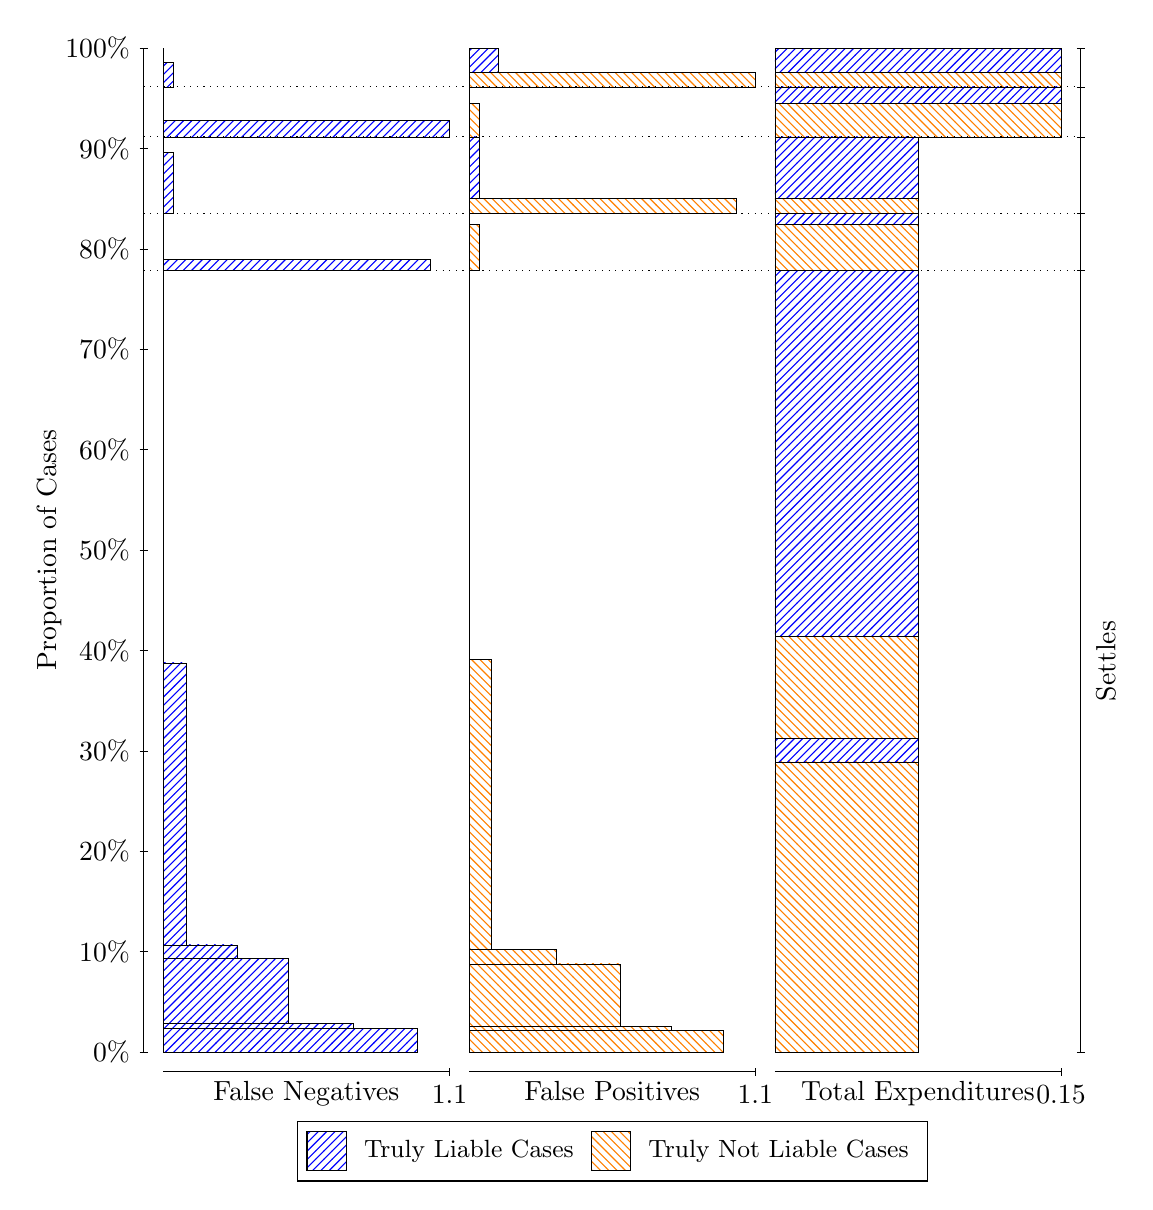
\begin{tikzpicture}
\draw[black, very thin] (1.5,1.75) -- (1.5,14.5);
\node[rotate=90, anchor=center] at (0.3, 8.125) {Proportion of Cases};
\draw[black, very thin] (1.45,1.75) -- (1.55,1.75);
\node[anchor=east] at (1.45, 1.75) {0\%};
\draw[black, very thin] (1.45,3.025) -- (1.55,3.025);
\node[anchor=east] at (1.45, 3.025) {10\%};
\draw[black, very thin] (1.45,4.3) -- (1.55,4.3);
\node[anchor=east] at (1.45, 4.3) {20\%};
\draw[black, very thin] (1.45,5.575) -- (1.55,5.575);
\node[anchor=east] at (1.45, 5.575) {30\%};
\draw[black, very thin] (1.45,6.85) -- (1.55,6.85);
\node[anchor=east] at (1.45, 6.85) {40\%};
\draw[black, very thin] (1.45,8.125) -- (1.55,8.125);
\node[anchor=east] at (1.45, 8.125) {50\%};
\draw[black, very thin] (1.45,9.4) -- (1.55,9.4);
\node[anchor=east] at (1.45, 9.4) {60\%};
\draw[black, very thin] (1.45,10.675) -- (1.55,10.675);
\node[anchor=east] at (1.45, 10.675) {70\%};
\draw[black, very thin] (1.45,11.95) -- (1.55,11.95);
\node[anchor=east] at (1.45, 11.95) {80\%};
\draw[black, very thin] (1.45,13.225) -- (1.55,13.225);
\node[anchor=east] at (1.45, 13.225) {90\%};
\draw[black, very thin] (1.45,14.5) -- (1.55,14.5);
\node[anchor=east] at (1.45, 14.5) {100\%};

\draw[black, very thin] (13.4,1.75) -- (13.4,14.5);
\draw[black, very thin] (13.35,1.75) -- (13.45,1.75);
\node[anchor=west] at (13.35, 1.75) {};
\draw[black, very thin] (13.35,11.679) -- (13.45,11.679);
\node[anchor=west] at (13.35, 11.679) {};
\draw[black, very thin] (13.35,12.397) -- (13.45,12.397);
\node[anchor=west] at (13.35, 12.397) {};
\draw[black, very thin] (13.35,13.372) -- (13.45,13.372);
\node[anchor=west] at (13.35, 13.372) {};
\draw[black, very thin] (13.35,14.006) -- (13.45,14.006);
\node[anchor=west] at (13.35, 14.006) {};
\draw[black, very thin] (13.35,14.5) -- (13.45,14.5);
\node[anchor=west] at (13.35, 14.5) {};

\draw[black, very thin, pattern color=blue, pattern=north east lines] (1.75,1.75) rectangle (4.9751,2.0449);
\draw[black, very thin, pattern color=blue, pattern=north east lines] (1.75,2.0449) rectangle (4.1586,2.1102);
\draw[black, very thin, pattern color=blue, pattern=north east lines] (1.75,2.1102) rectangle (3.5054,2.1114);
\draw[black, very thin, pattern color=blue, pattern=north east lines] (1.75,2.1114) rectangle (3.3421,2.9372);
\draw[black, very thin, pattern color=blue, pattern=north east lines] (1.75,2.9372) rectangle (2.689,3.1099);
\draw[black, very thin, pattern color=blue, pattern=north east lines] (1.75,3.1099) rectangle (2.0358,6.6927);
\draw[black, very thin, pattern color=orange, pattern=north west lines] (1.75,6.6927) rectangle (1.75,11.679);
\draw[black, very thin, pattern color=blue, pattern=north east lines] (1.75,11.679) rectangle (5.1384,11.815);
\draw[black, very thin, pattern color=orange, pattern=north west lines] (1.75,11.815) rectangle (1.75,12.397);
\draw[black, very thin, pattern color=blue, pattern=north east lines] (1.75,12.397) rectangle (1.8725,13.175);
\draw[black, very thin, pattern color=orange, pattern=north west lines] (1.75,13.175) rectangle (1.75,13.372);
\draw[black, very thin, pattern color=blue, pattern=north east lines] (1.75,13.372) rectangle (5.3833,13.577);
\draw[black, very thin, pattern color=orange, pattern=north west lines] (1.75,13.577) rectangle (1.75,14.006);
\draw[black, very thin, pattern color=blue, pattern=north east lines] (1.75,14.006) rectangle (1.8725,14.319);
\draw[black, very thin, pattern color=orange, pattern=north west lines] (1.75,14.319) rectangle (1.75,14.5);
\draw[black, very thin, pattern color=orange, pattern=north west lines] (5.6333,1.75) rectangle (8.8584,2.0205);
\draw[black, very thin, pattern color=orange, pattern=north west lines] (5.6333,2.0205) rectangle (8.2052,2.0745);
\draw[black, very thin, pattern color=orange, pattern=north west lines] (5.6333,2.0745) rectangle (7.5521,2.8685);
\draw[black, very thin, pattern color=orange, pattern=north west lines] (5.6333,2.8685) rectangle (7.3888,2.8695);
\draw[black, very thin, pattern color=orange, pattern=north west lines] (5.6333,2.8695) rectangle (6.7356,3.052);
\draw[black, very thin, pattern color=orange, pattern=north west lines] (5.6333,3.052) rectangle (5.9191,6.736);
\draw[black, very thin, pattern color=blue, pattern=north east lines] (5.6333,6.736) rectangle (5.6333,11.679);
\draw[black, very thin, pattern color=orange, pattern=north west lines] (5.6333,11.679) rectangle (5.7558,12.261);
\draw[black, very thin, pattern color=blue, pattern=north east lines] (5.6333,12.261) rectangle (5.6333,12.397);
\draw[black, very thin, pattern color=orange, pattern=north west lines] (5.6333,12.397) rectangle (9.0217,12.593);
\draw[black, very thin, pattern color=blue, pattern=north east lines] (5.6333,12.593) rectangle (5.7558,13.372);
\draw[black, very thin, pattern color=orange, pattern=north west lines] (5.6333,13.372) rectangle (5.7558,13.801);
\draw[black, very thin, pattern color=blue, pattern=north east lines] (5.6333,13.801) rectangle (5.6333,14.006);
\draw[black, very thin, pattern color=orange, pattern=north west lines] (5.6333,14.006) rectangle (9.2667,14.187);
\draw[black, very thin, pattern color=blue, pattern=north east lines] (5.6333,14.187) rectangle (6.0007,14.5);
\draw[black, very thin, pattern color=orange, pattern=north west lines] (9.5167,1.75) rectangle (11.333,5.4341);
\draw[black, very thin, pattern color=blue, pattern=north east lines] (9.5167,5.4341) rectangle (11.333,5.7289);
\draw[black, very thin, pattern color=orange, pattern=north west lines] (9.5167,5.7289) rectangle (11.333,7.0309);
\draw[black, very thin, pattern color=blue, pattern=north east lines] (9.5167,7.0309) rectangle (11.333,11.679);
\draw[black, very thin, pattern color=orange, pattern=north west lines] (9.5167,11.679) rectangle (11.333,12.261);
\draw[black, very thin, pattern color=blue, pattern=north east lines] (9.5167,12.261) rectangle (11.333,12.397);
\draw[black, very thin, pattern color=orange, pattern=north west lines] (9.5167,12.397) rectangle (11.333,12.593);
\draw[black, very thin, pattern color=blue, pattern=north east lines] (9.5167,12.593) rectangle (11.333,13.372);
\draw[black, very thin, pattern color=orange, pattern=north west lines] (9.5167,13.372) rectangle (13.15,13.801);
\draw[black, very thin, pattern color=blue, pattern=north east lines] (9.5167,13.801) rectangle (13.15,14.006);
\draw[black, very thin, pattern color=orange, pattern=north west lines] (9.5167,14.006) rectangle (13.15,14.187);
\draw[black, very thin, pattern color=blue, pattern=north east lines] (9.5167,14.187) rectangle (13.15,14.5);
\draw[black, dotted] (1.5,11.679) -- (13.4,11.679);
\draw[black, dotted] (1.5,12.397) -- (13.4,12.397);
\draw[black, dotted] (1.5,13.372) -- (13.4,13.372);
\draw[black, dotted] (1.5,14.006) -- (13.4,14.006);
\draw[black, very thin] (1.75,1.5) -- (5.3833,1.5);
\node[anchor=north] at (3.5667, 1.5) {False Negatives};
\draw[black, very thin] (5.3833,1.45) -- (5.3833,1.55);
\node[anchor=north] at (5.3833, 1.45) {1.1};

\draw[black, very thin] (5.6333,1.5) -- (9.2667,1.5);
\node[anchor=north] at (7.45, 1.5) {False Positives};
\draw[black, very thin] (9.2667,1.45) -- (9.2667,1.55);
\node[anchor=north] at (9.2667, 1.45) {1.1};

\draw[black, very thin] (9.5167,1.5) -- (13.15,1.5);
\node[anchor=north] at (11.333, 1.5) {Total Expenditures};
\draw[black, very thin] (13.15,1.45) -- (13.15,1.55);
\node[anchor=north] at (13.15, 1.45) {0.15};

\node[black, centered, rotate=90] at (13.72, 6.7144) {Settles};





\draw (7.449999999999999,1.5) node[draw=none] (baseCoordinate) {};
\begin{scope}[align=center]
        \matrix[scale=0.5, draw=black, below=0.5cm of baseCoordinate, nodes={draw}, column sep=0.1cm]{
            \node[rectangle, draw, minimum width=0.5cm, minimum height=0.5cm, pattern=north east lines, pattern color=blue] {}; &
            \node[draw=none, font=\small] (B) {Truly Liable Cases}; &
            \node[rectangle, draw, minimum width=0.5cm, minimum height=0.5cm, pattern=north west lines, pattern color=orange] {}; &
            \node[draw=none, font=\small] (B) {Truly Not Liable Cases}; \\
            };
\end{scope}

\end{tikzpicture}
\end{document}